\documentclass{article}

\usepackage{pdfpages}
\usepackage[nottoc]{tocbibind}
\usepackage{color}
\usepackage{wrapfig}
\usepackage{graphicx}
\usepackage{subcaption}
\graphicspath{ {../plots/} }
\usepackage{tikz}
\usetikzlibrary{calc,positioning,arrows}
\usepackage{amsmath,amsthm}


\iffalse
\newcommand{\comment}[1]{\textit{\textcolor{blue}{/* #1 */} }}
\fi
\newcommand{\todo}[1]{\textit{\textcolor{red}{// TODO: #1} }}
\newcommand{\draft}[1]{\textit{\textcolor{olive}{#1} }}
\newcommand{\code}[1]{\texttt{#1}}


\theoremstyle{plain}
\newtheorem{thm}{Theorem}[section]
\newtheorem{lem}[thm]{Lemma}
\newtheorem{prop}[thm]{Proposition}
\newtheorem*{cor}{Corollary}

\theoremstyle{definition}
\newtheorem{defn}{Definition}[section]
\newtheorem{conj}{Conjecture}[section]
\newtheorem{exmp}{Example}[section]

\theoremstyle{remark}
\newtheorem*{rem}{Remark}
\newtheorem*{note}{Note}

\begin{document}
\iffalse
\fi


\tableofcontents
\pagebreak
\section{Introduction}
\todo{What are we doing. Why are we doing this}

\pagebreak
\section{Background}
\todo{Fairly detailed section on rdma / ibverbs. Explain all verbs.}


\pagebreak
\section{Related Work}

\todo{Overview of related papers. Include different benchmark papers}

\todo{Maybe also include systems using rdma protocols. Compare to our findings. Should they have used other connection? 
Maybe add this after the protocols section?}

\pagebreak
\section{Performance Model}\label{sec:perf-model} \label{sec:model}
In this section we introduce a general performance model for data exchange protocol that will allow us to estimate the 
performance of our protocol implementations. It gives us a better understanding of our evaluation results and helps us 
to locate bottlenecks.

\paragraph{}We took a fairly detailed look at the operations involved in transmitting a message using RDMA in Section~\ref{sec:rdma}.
Trying to closely model this however gives us a far too complex model, with a lot of parameters that are hard to assess,
especially if we start to look at more complex protocols. We introduce a more simplified model inspired by the  
\emph{LogGP model}~\cite{loggp}, which was developed  to model point to point communication with variable message sizes for 
traditional IP based networks.

\paragraph{} At its core the LogGP model uses a fixed CPU overhead $o$ per message, the communication latency $L$, and 
the bandwidth $G$. While this results in a decent model for IP based system, it is unable to model the heavy NIC offloading 
happening in RDMA. We extended the LogGP model by splitting the offset $o$ into multiple offsets for each of the components.
We also largely ignored the number of processes $P$ and use a slightly different definition for the gap $g$. This leaves 
us with the following parameters, which are illustrated in Figure~\ref{fig:model-base}.

\begin{figure}[!htp]
\begin{center}
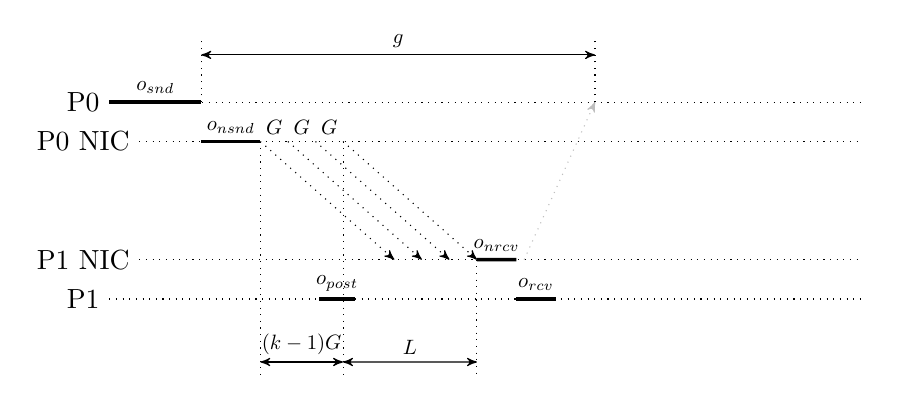
\begin{tikzpicture}[node distance=1cm,auto,>=stealth']
  \node[] (p0) {P0};
  \node[right of=p0, node distance=10cm] (p0_g) {};
  \draw[dotted] (p0) -- (p0_g);

  \node[below of=p0, node distance=0.5cm] (p0_nic) {P0 NIC};
  \node[right of=p0_nic, node distance=10cm] (p0_nic_g) {};
  \draw[dotted] (p0_nic) -- (p0_nic_g);

  \node[below of=p0_nic, node distance=1.5cm] (p1_nic) {P1 NIC};
  \node[right of=p1_nic, node distance=10cm] (p1_nic_g) {};
  \draw[dotted] (p1_nic) -- (p1_nic_g);

  \node[below of=p1_nic, node distance=0.5cm] (p1) {P1};
  \node[right of=p1, node distance=10cm] (p1_g) {};
  \draw[dotted] (p1) -- (p1_g);
  

  %%%%

  \draw[very thick] (p0) --node[above,scale=0.75,midway]{$o_{snd}$} ($(p0)!0.15!(p0_g)$);
  \draw[very thick] ($(p0_nic)!0.15!(p0_nic_g)$) --node[above,scale=0.75,midway]{$o_{nsnd}$} ($(p0_nic)!0.225!(p0_nic_g)$);


  \path[] ($(p0_nic)!0.225!(p0_nic_g)$) --node[above,scale=0.75,midway]{$G$} ($(p0_nic)!0.26!(p0_nic_g)$);
  \draw[dotted, ->] ($(p0_nic)!0.225!(p0_nic_g)$) -- ($(p1_nic)!0.395!(p1_nic_g)$);

  \path[] ($(p0_nic)!0.26!(p0_nic_g)$) --node[above,scale=0.75,midway]{$G$} ($(p0_nic)!0.295!(p0_nic_g)$);
  \draw[dotted, ->] ($(p0_nic)!0.26!(p0_nic_g)$) -- ($(p1_nic)!0.43!(p1_nic_g)$);

  \path[] ($(p0_nic)!0.295!(p0_nic_g)$) --node[above,scale=0.75,midway]{$G$} ($(p0_nic)!0.33!(p0_nic_g)$);
  \draw[dotted, ->] ($(p0_nic)!0.295!(p0_nic_g)$) -- ($(p1_nic)!0.465!(p1_nic_g)$);

  \draw[dotted, ->] ($(p0_nic)!0.33!(p0_nic_g)$) -- ($(p1_nic)!0.5!(p1_nic_g)$);


  \draw[very thick] ($(p1_nic)!0.5!(p1_nic_g)$) --node[above,scale=0.75,midway]{$o_{nrcv}$} ($(p1_nic)!0.55!(p1_nic_g)$);
  \draw[very thick] ($(p1)!0.30!(p1_g)$) --node[above,scale=0.75,midway]{$o_{post}$} ($(p1)!0.345!(p1_g)$);
  \draw[very thick] ($(p1)!0.55!(p1_g)$) --node[above,scale=0.75,midway]{$o_{rcv}$} ($(p1)!0.6!(p1_g)$);
    
  %%%%

  \draw[dotted] ($(p0_nic)!0.225!(p0_nic_g)$) -- ($(p0_nic)!0.225!(p0_nic_g)+(0,-3)$);
  \draw[dotted] ($(p0_nic)!0.330!(p0_nic_g)$) -- ($(p0_nic)!0.330!(p0_nic_g)+(0,-3)$);
  \draw[<->] ($(p0_nic)!0.225!(p0_nic_g)+(0,-2.8)$) --node[above,scale=0.75,midway]{$(k-1)G$} ($(p0_nic)!0.330!(p0_nic_g)+(0,-2.8)$);

  \draw[dotted] ($(p1_nic)!0.5!(p1_nic_g)$) -- ($(p1_nic)!0.5!(p1_nic_g)+(0,-1.5)$);
  \draw[<->] ($(p0_nic)!0.330!(p0_nic_g)+(0,-2.8)$) --node[above,scale=0.75,midway]{$L$} ($(p1_nic)!0.5!(p1_nic_g)+(0,-1.3)$);


  \draw[dotted] ($(p0)!0.15!(p0_g)$) -- ($(p0)!0.15!(p0_g)+(0,.8)$);
  \draw[dotted] ($(p0)!0.65!(p0_g)$) -- ($(p0)!0.65!(p0_g)+(0,.8)$);
  \draw[<->] ($(p0)!0.15!(p0_g)+(0,.6)$) --node[above,scale=0.75,midway]{$g$} ($(p0)!0.65!(p0_g)+(0,.6)$);

  %%%%

  \draw[dotted, ->, lightgray] ($(p1_nic)!0.56!(p1_nic_g)$) -- ($(p0)!0.65!(p0_g)$);


\end{tikzpicture}
\end{center}
\caption{Sending an receiving messages under our model}
\label{fig:model-base}
\end{figure}




\begin{itemize}
  \item $L$: the network Latency, incurred by sending a message from the senders NIC to the receivers NIC. In our model 
    this also includes the PCI latency.
  \item $G$: the gap per byte for long messages. For our purposes this is the time of sending a single byte given the 
    maximum bandwidth of our link.
  \item $o_{snd}$: the \emph{send overhead}, defined as the length of time that a processor is engaged in sending each message.
    For some protocols this also includes any preparation and communication overhead necessary to send a message.
  \item $g$: the \emph{send gap}, defined as the minimum time interval until the sender can reuse the resources involved in 
    the transmission. (e.g. the send buffer) 
  \item $o_{nsnd}$: the \emph{send NIC overhead}, defined as the length of time that a NIC is engaged in sending each message.
  \item $o_{nrcv}$: the \emph{receive NIC overhead}, defined as the length of time that a NIC is engaged in receiving each message.
  \item $o_{rcv}$: the \emph{receive overhead}, defined as the length of time that a processor is engaged in receiving each message.
  \item $o_{post}$: the \emph{posting overhead}, defined as the time that a processor is engaged in preparing a receive buffer
    to receive into (e.g. post receive). This needs to happen sometime before receiving the next message.
\end{itemize}

\paragraph{} This model does not take the MTU into account. While some prior work use a slightly different model when sending 
messages over the MTU, that span multiple transmission units~\cite{dare}, we found our model to works well enough to understand
most of our results.

\paragraph{} We built this model around send or write based protocols and it was not designed 
for read based protocols. But as we will see it can still give us better insight in the observed performance of these 
protocols.

\paragraph{} Even with these simplifications it still is a fairly complex model and measuring each of these overheads in 
practice is very hard. We do not try to quantitatively evaluate our model for all presented protocols, but rather use it 
get a better general understanding of the observed performance characteristics and to understand what is limiting throughput
or latency in which situations.

\pagebreak
\subsection{Evaluating the Model}

\paragraph{} In this section we evaluate the model for the send-receive protocol only. Table~\ref{tab:model} shows our model
parameter estimates. 

\begin{table}[!ht]
\setlength\tabcolsep{1.5pt}
\centering
\caption{Model parameter for send-receive protocol}
\label{tab:model}
\begin{threeparttable}[t]
 \begin{tabular}{|x{3.5cm}|x{3.5cm}|x{3.5cm}|} % I specify the sizes of columns. x is for centering and p is  for left
 \hline
 Parameter    &  single & batched \\
  \hline
  \hline
 $o_{snd}$    & $0.12 \mu s$ &  $0.016 \mu s$\\
  \hline
 $o_{rcv}$    & $0.052 \mu s$ & $0.017 \mu s$\\
  \hline
 $o_{post}$   & $0.016 \mu s$ & $0.007 \mu s$\\
  \hline
 $o_{nsnd}$   & $0.02 \mu s$\tnote{a} &  \cellcolor{black!40} \\
  \hline
 $o_{nrcv}$   & $0.02 \mu s$\tnote{a} &  \cellcolor{black!40} \\
  \hline
 $L$          & $1.9 \mu s$ &  \cellcolor{black!40}\\
  \hline
 $g$          & $\geq 3.4 \mu s$\tnote{b}  & \cellcolor{black!40}\\
 \hline
 $G$          & $0.2\mu s / KB$  & $0.084\mu s / KB$\\

\hline
\end{tabular}
\begin{tablenotes}
\item[a] \small The on NIC overheads are expected to be very small and are hard to accurately measure
\item[b] \small Very protocol dependent. Increases linearly for the send-receive protocol
\end{tablenotes}
\end{threeparttable}
\end{table}


\paragraph{} We are able to directly measure $o_{snd}$, $o_{rcv}$, and $o_{post}$. For the send-receive protocol $o_{snd}$ is the cost of 
posting a single send request. The receiving overhead $o_{rcv}$ is the cost of polling for a receive completion event. And
$o_{post}$ is the cost for posting a single receive request. For all of these overheads we measure both the cost of a single
operation, as well as the cost per message when issuing multiple operations in a batch.

\paragraph{} The gap $g$ is also directly measurable. This is the time it takes until the send is completed and has been
acknowledged. The lower bound for this is at $3.4\mu s$, or a bit less then twice the network latency L. But it increases
linearly with the size of the message $k$.

It is worth noting here, that our reported network latency $L$ includes both the PCI latency as well as the latency
of the switch between our two nodes.

\paragraph{} For the network bandwidth G we also report a batched and unbatched estimation. We use the unbatched estimation
for our latency prediction and the batched estimation for our throughput predictions.

\paragraph{} Evaluating the RNIC overhead is tricky. We make the assumption that $o_{nsnd} = o_{nrcv}$ and use our latency
and bandwidth measurement to estimate these parameters. This gives us a good enough estimation for a 1:1 communication pattern.




\paragraph{} While we will see that our model is not quite able to accurately predict our bandwidth and latency 
measurements, it does  give us a better understanding of our results and predicts the different types of bottlenecks 
we encounter in our evaluation.

\subsubsection{Predicting Latency}

Predicting latency using our model essentially means evaluating the parameters in the critical path and adding them up. 
The predicted latency $t$ of transferring a single message of size $k$ is:

$$
t \geq o_{snd} + o_{nsnd}  + (k-1)G + L + o_{nrcv} + o_{rcv}
$$


\begin{figure}[ht]
  \centering
  \includegraphics[width=1\textwidth]{send-lat-msgsize.png}
  \caption{Send-Receive latency and model prediction}
    \label{fig:model-lat}
\end{figure}

\paragraph{} Figure~\ref{fig:model-lat} shows our prediction and the actual latency measurements for the send-receive protocol.
We can see that we are not quite able to precisely match the actual data. It does
however confirm our prediction of a mostly linear increase in latency with increased message size.


\subsubsection{Predicting Bandwidth}
Predicting maximum bandwidth is not quite as simple as adding up all parameters. The model predicts three different kinds of
bottlenecks. We take a look at each of these bottlenecks and illustrate them on the send-receive protocol in Figure~\ref{fig:model-bw}.

\begin{figure}[ht]
  \centering
  \includegraphics[width=1\textwidth]{send-bw-msgsize.png}
  \caption{Send-Receive bandwidth and model prediction}
    \label{fig:model-bw}
\end{figure}

\paragraph{Round-Trip bottleneck} One way to be bottlenecked is by simply not issuing enough concurrent send requests. In 
this case we are bottlenecked by the gap $g$, which usually contains a complete round-trip time and grows linearly with 
the size of the message. So when we issue only a single send at a time, for a message size of $k$ we predict to be limited by

$$
bw \leq \frac{k}{o_{snd} + g}\text{, where } g = g_{fix} + kg_{var} 
$$

For the send-receive protocol this is exactly what we see. SR-Seq shows the throughput with varying message size when only 
sending a single message at a time. 

\paragraph{} This means to get decent 1:1 performance it is vitally important to issue enough concurrent requests, or as we 
will call it from now on to allow for enough \emph{unacknowledged} messages. In a lot of related work this is not discussed
and either done without specifically mentioning it or sometimes the presented protocol only allows for a single unacknowledged
message, without bringing up the disadvantages of such an approach.


\paragraph{CPU bottleneck} Another bottleneck we encounter especially for small messages, is a CPU bottleneck, either at the 
sender or receiver.

A sending CPU bottleneck means we simply are not able to issue enough send requests and the RNIC is processing them faster
than we post them. This results in a predicted limit of

$$
bw \leq \frac{k}{o_{snd}}
$$


The send-receive protocol (SR) allows for multiple unacknowledged messages and avoid the previous bottleneck. 
This implementations is limited by a sending CPU bottleneck. In Figure~\ref{fig:model-bw} we can see the linearly
increasing throughput we predict until we reach a message size of 2 KB where we start to be limited by the NIC.

\paragraph{} We can avoid this bottleneck by introducing batching. The verbs API allows us to post multiple work request at 
the same time. This \emph{Doorbell batching} reduces the number of generated MMIOs~\cite{anuj-guide} and reduces the CPU load.
We measured that batching can reduce the sending CPU overhead $o_{snd}$ by up to a factor of 10. 

When introducing doorbell batching to the send-receive protocol we never seem to be bottlenecked by the sending CPU as 
can be seen for the batched measurement SR-Bat in Figure~\ref{fig:model-bw}.
Although this can drastically improve bandwidth, we will not evaluate other protocols with doorbell batching, as it is
not directly applicable to some of the protocols and for connected QPs application level batching, i.e. sending larger 
messages, is a better approach.

\paragraph{} A receiving CPU bottleneck means the receiver is unable to prepare enough receive buffers, staling the sender. 
This gives us a predicted limit of

$$
bw \leq \frac{k}{o_{rcv} + o_{post}}
$$

This results in a very similar bottleneck which is proportional to the message size. We do not encounter this bottleneck for
our 1:1 evaluation of the send-receive protocol, however when a single receiving thread handles multiple open connection 
in a N:1 communication pattern this quickly becomes the key bottleneck.

Similarly to the sending CPU bottleneck the impact can be reduced using batching.


\paragraph{Device Bottleneck} Finally if we are able to issue enough requests, and the receiver is not stalling the sender,
we are bottlenecked by either one of the involved RNICs. According to our model this results in one of these two limits

$$
bw \leq \frac{k}{o_{nsnd} + (k-1)G} \text{\quad or \quad} bw \leq \frac{k}{o_{nrcv} + (k-1)G}
$$

In both cases with increasing message size we first predict a linear increase in bandwidth which will eventually 
flatten out into the maximum possible goodput of the network link.

Looking at the batched throughput results SR-Bat in Figure~\ref{fig:model-bw}, this is qualitatively what we expect 
when being only limited by the RNIC. We are however not able to accurately predict the results for smaller messages 
using our current model. This is a limitation of our model,  possibly caused by not modeled hardware optimizations.


\pagebreak
\section{Protocols}
\todo{Look at all implemented protocols. Detailed description of the protocols. Add performance model for each of them and provide benchmarks.}

\pagebreak
\section{Send Receive} \label{sec:conn:send}\label{sendrcv}\label{sendrcv-design}

The send-receive protocol is by far the simplest, as the send and receive verbs already provide the required 
message passing interface. There are still multiple ways to implement and optimize such a protocol and a few pitfalls 
we need to address to get good performance.

\paragraph{} We presented the basic function of the send verb in Section \ref{sec:bg:send}. It allows the sender to transmit 
a message to the receiver, without any additional information, as long as the receiver has posted a receive buffer that is 
large enough to receive the message. To transform this verb to a fully functioning connection, we add two basic things. 
A kind of \emph{receive buffer management} that allows the receiver to receive multiple messages at the same time, 
and to get any reasonable performance we need to be able to send multiple messages asynchronously.

\subsection{Protocol} 

The sender assumes that the receiver is always ready to receive the message and has at least one receive buffer 
posted. This means sending essentially only involves issuing a send work request. As we already mentioned earlier, it is very 
important to keep the sending pipeline full to get good performance. Using \emph{unacknowledged messages} can increase
throughput by a factor of five or more.
We use the trick of issuing send requests with monotonically increasing \code{wr\_id}s, explained in Section~\ref{sec:protocols},
to be able to support multiple 
outstanding messages.

\paragraph{} The receiver always needs to have at least one posted receive buffer. We achieve this by having an array of 
posted receive buffers, which are initially registered during connection setup. When receiving a new message we return 
the corresponding buffer. We can match a completion event to the correct buffer by using the array index of the receive 
buffer as a \code{wr\_id} when posting the receive request. As soon as the application is done processing the message,
it marks it as free which will repost the corresponding buffer. By having multiple receive buffers it allows us to have 
numerous unacknowledged messages which improves performance drastically.

\paragraph{} It is important to note that in production systems there needs to be a way for the sender to notice whether 
enough receive buffers are ready. If there is no posted receive buffer available when a message is received,
the receiver  generates
a so-called \emph{Reader Not Ready} error. This will either cause a large back-off for the sender 
or even cause the connection
to break.

We observed this problem specifically for N:1 communication. This can be mitigated to some extend by optimizing receiving and
reposting buffers.




\subsection{Extensions}

There are multiple extensions to the described base protocol. The changes either improve performance, allow us to
share resources between connections, or enable different kinds of communication patterns.

\subsubsection{Inline Sending}
The send verb has a slight variation called \emph{inline send}. Inline sending means that instead of 
simply referencing the payload in a work request, the sending CPU directly copies it to the RNIC using MMIO. This prevents
the NIC from having to issue an addition DMA and can reduce latency for very small messages~\cite{anuj-guide}. It does,
however,
increase the load for the sending CPU. As we will see, the sending CPU is oftentimes the bottleneck so we did not further 
evaluate inline sending in this thesis. It can, however, be a viable optimization for small messages.


\subsubsection{Receive Batching} 
As described, there are significant penalties if the receiver is not able to keep up and stalls the sender.
This can be mitigated a little by optimizing the receiver. For one, instead of polling one receive CQ at a time we poll up to 32
at a time into an array of CQEs. We observed in microbenchmarks that this can improve the observed throughput by nearly half.
And by batching the reposting of receive buffers we can also further improve throughput.

\subsubsection{Shared Receive Queues} 
By having an array of $k$ posted receive buffers for each receiver, the memory reserved for receiving messages can grow quite
large. If a node has  open connections to $N$ other nodes, it needs to reserve  $N*k*max\_msg\_size$ bytes, even if 
the total request volume is quite small (i.e., we expect only burst of $k$ messages but from different nodes at different times).

We can reduce the total memory usage by using \emph{Shared Receive Queues~(SRQ)}. As the name already tells us SRQs allow us
to share receive queues between multiple QPs. This means, we can reuse a single receive queue
for multiple connections, allowing
multiple receivers to share the same receive buffers. This means the total memory usage does not grow with the number of
open connections, but stays constant.

The usage of SRQs does not impact completion queues. The completion event for consuming a posted receive buffer still ends up 
in the CQ of the corresponding QP.

One major change when using an SRQ is that we do not submit receive work requests to the respective QPs but to the single SRQ. This
means that we either have to introduce locking to access the SRQ, which introduces a significant performance penalty, or 
delegate the posting of the receive buffer to a single thread. Instead of reposting the buffer themselves, each connection 
enqueues the id of the to be posted buffer into a queue. The single reposting thread will dequeue and repost it. This also
allows us to have central batching for reposting the buffers. We opted to use the latter approach for our SRQ based 
implementation.

\subsubsection{Single Receiver} 
It is very common to have an N:1 communication pattern where a single server receives messages from multiple clients. This
could be achieved by simply round-robin over the $N$ connections. For this connection, however, we used the fact that we can 
associate a single completion queue with multiple queue pairs. This means, if we are in a \emph{single receiver mode}, all 
receive completion events will end up in a single CQ. Allowing us to poll a single queue to receive a message from $N$ 
different sender.


\subsection{Feature Analysis}

The Send and Receive verbs are generally regarded as the simplest verbs to work with and they give us a lot of features
that make them suitable for many applications. We take a look at the traits we introduced in Section~\ref{sec:features} 
and see which of them are met by our send-receive protocol.

\paragraph{} The protocol fulfills our requirements for being \emph{non-blocking}, which means if the receiving application does not free a single
received buffer, it does not impact the protocols ability to transmit new messages.
It also provides us with convenient \emph{interrupts} that allow us to save a lot CPU utilization for certain workloads.
Finally, when using shared receive queues, the protocol allows us to \emph{share resources} between multiple connections.

\paragraph{} It does, however, not allow for \emph{variable message sizes} which can unnecessarily blow up the total memory
requirements if an application needs to send many small and a few large messages, as each of the small messages will have
to consume a buffer that is large enough to contain a large message. We also argue that the protocol is not truly 
\emph{zero copy} as for almost all real world use cases we would need to copy the received message out of the
receive buffer and into a data structure.



\pagebreak
\section{Buffered Write} \label{sec:conn:buf_write}

\subsection{Design}
As described in Section \ref{sec:proto-ds} there are many different ways to implement a buffer write protocol, or a
protocol that writes to a ring buffer. We decided that we want to allow for variable message sizes. That means 
in contrast to the send protocol presented in section \ref{sec:conn:send} we do not have a fixed maximum buffer size
that will always be consumed, but we will only use the space we actually need.

\paragraph{} As we discussed we have two distinct problems we need to solve to get a correct buffered write connection.

\begin{itemize}
  \item We need to signal to the receiver that we have written to the buffer and how much was written. This is tightly 
    coupled to \emph{how} we write the data. We implemented three different approaches for solving this, which we present
    in the \emph{Sending} section below.
  \item We need to signal to the sender whether there is enough space to write the message. We implemented both a \emph{push}
    and \emph{pull} based implementation in the \emph{Acknowledging} section below.
\end{itemize}


\subsubsection{Buffer} \label{sec:conn:write:buf}
\begin{figure}[!ht]
\begin{center}

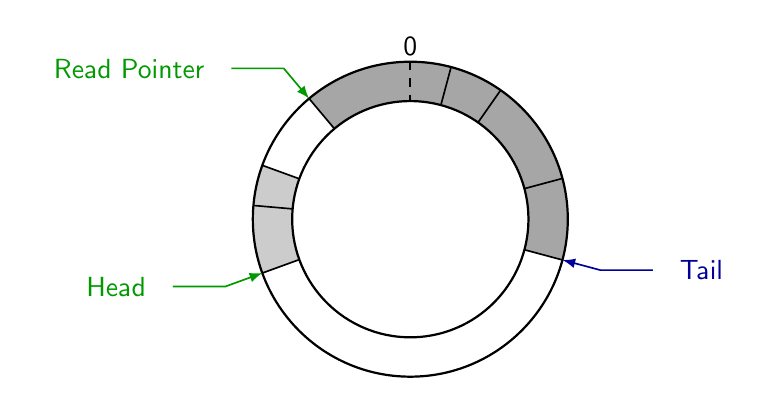
\begin{tikzpicture}[>=latex,font=\sffamily,semithick,scale=2]
    \fill [black!35] (0,0) -- (130:1) arc [end angle=-15, start angle=130, radius=1] -- cycle;

    \fill [black!20] (0,0) -- (200:1) arc [end angle=160, start angle=200, radius=1] -- cycle;
    \draw [thick] (0,0) circle (1cm);

    \node (zero) at (90:1.1) {0};
    \draw[dashed] (90:1) -- (0:0);
    \draw (200:1) -- (0:0);
    \draw (175:1) -- (0:0);
    \draw (160:1) -- (0:0);

    \draw (130:1) -- (0:0);
    \draw (75:1) -- (0:0);
    \draw (55:1) -- (0:0);
    \draw (15:1) -- (0:0);
    \draw (-15:1) -- (0:0);
    \node [circle,thick,fill=white,draw=black,align=center,minimum size=3cm] at (0,0) {};


    \draw [<-,black!40!green] (130:1) -- (130:1.25) -- +(-.333,0)
        node [black!40!green,left,inner xsep=.333cm] (rptr) {Read Pointer};
    \draw [<-,black!40!green] (200:1) -- (200:1.25) -- +(-.333,0)
        node [black!40!green,left,inner xsep=.333cm] (Head) {Head};
    \draw [<-,black!40!blue] (-15:1) -- (-15:1.25) -- +(.333,0)
        node [black!40!blue,right,inner xsep=.333cm] (Tail) {Tail};
\end{tikzpicture}

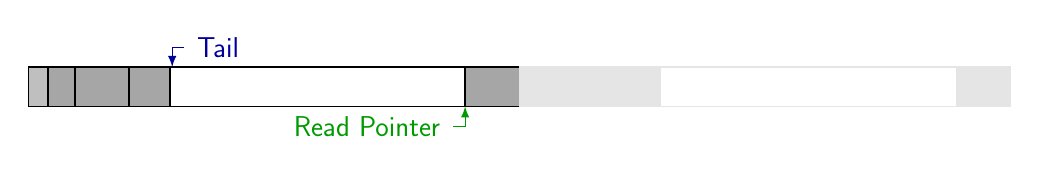
\begin{tikzpicture}[>=latex,font=\sffamily,every node/.style={minimum width=1cm,minimum height=1cm,outer sep=0pt,draw=black,semithick, scale=0.5}]
        \node [minimum width=.5cm, fill=black!25] at (0,0) (A) {};
        \node [anchor=west, minimum width=.68cm, fill=black!35] at (A.east) (B) {};
        \node [anchor=west, minimum width=1.38cm, fill=black!35] at (B.east) (C) {};
        \node [anchor=west, minimum width=1.03cm, fill=black!35] at (C.east) (D) {};
        \node [anchor=west, minimum width=7.5cm] at (D.east) (E) {};

        \node [anchor=west, minimum width=1.38cm, fill=black!35] at (E.east) (F) {};

        \node [anchor=west, minimum width=.5cm, fill=black!10, draw=none] at (F.east) (A') {};
        \node [anchor=west, minimum width=.68cm, fill=black!10, draw=none] at (A'.east) (B') {};
        \node [anchor=west, minimum width=1.38cm, fill=black!10, draw=none] at (B'.east) (C') {};
        \node [anchor=west, minimum width=1.03cm, fill=black!10, draw=none] at (C'.east) (D') {};
        \node [anchor=west, minimum width=7.5cm, draw=none] at (D'.east) (E') {};
        \node [anchor=west, minimum width=1.38cm, fill=black!10, draw=none] at (E'.east) (F') {};
        \node [anchor=west, minimum width=12.47cm, draw=black!10] at (F.east) (A') {};

        \draw [<-,black!40!blue, scale=1] (1.7,.25) -- (1.7, .5)  -- +(.15,0)
        node [black!40!blue,right,inner xsep=.333cm, draw=none] (Tail) {\huge Tail};
        \draw [<-,black!40!green, scale=1] (5.42,-.25) -- +(0, -.25)  -- +(-.15,-.25)
        node [black!40!green,left,inner xsep=.333cm, draw=none] (Head) {\huge Read Pointer};

\end{tikzpicture}
\end{center}
\caption{Ring Buffer with twice mapped memory to allows DMA writes over the end}
\comment{Fix figure to include read pointer correctly}
\label{fig:ringbuffer}
\end{figure}

The core of our buffered read connection is a ring buffer. This buffer ensures that the sender always knows \emph{where} to 
write to. Figure \ref{fig:ringbuffer} shows the basis for our ring buffer that we use for all implementations.

\paragraph{} We use a buffer that allows us to write arbitrary message sizes. There are three relevant pointers. 
The \emph{tail} which points to the next free memory address, the \emph{head}, which points to  the end of the 
free memory region, and the \emph{read pointer} which points to the start of the next unprocessed message. 

\paragraph{} The tail is only stored and updated by the sender. The tail directly gives the sender the address to write the 
next message to. The only thing the sender needs to check is, if there is actually enough space in the buffer for the 
intended message. So it needs at least a semi regular update on the head position. We look into this problem in 
the \emph{Acknowledging} section below.

\paragraph{} Receiving is a little more involved. Similarly to how we implemented the receive buffer management in 
Section \ref{sec:conn:send} we want to have the notion of \emph{reading} which returns a pointer to the start of 
the next unread message and \emph{freeing} a message which allows us to reuse that section of the ring buffer. 

This is where the difference between the \emph{head} and the \emph{read pointer} becomes apparent. The read pointer points 
to the next message the receiver has not read, while the head points to the oldest message the receiver has not freed. Reading
and freeing messages should work while interleaving, so we need some kind of management of free buffer to update the head 
correctly.

We solve this in a very simple way by having a linked list containing the starting address of the received messages. When
reading we push the address to the end of the list. When freeing we remove it from the list. The head is always the first 
element in the list.

We should note that the length of the message has to be communicated in some way, which we will address in the section 
\emph{Sending} below.





\paragraph{"Magic" Buffer} One problem we encountered while using such a ring buffer for RDMA is that we cannot simply 
\emph{wrap around} the end of the buffer using DMA. So if we want to write a message that is larger then the space left until
the end of the buffer we either need to skip to the front of the buffer, wasting space, or perform two writes, which is 
significantly slower.

Figure \ref{fig:ringbuffer} shows the our problem. Message $A$ cannot be written in a single RDMA write as it consists of 
two distinct, not connected memory regions. We can solve this by using something that has been coined 
\emph{"Magic" ring buffer} \comment{By? rgiesen.wordpress.com? Someone else?}. The idea is to map the same physical twice,
so that the same physical memory is adjacent to itself in virtual memory. You can see a representation of this in the 
Figure above. We use \emph{shared memory segments} on Linux to achieve this memory layout.

With this change we can simply write over the end of the buffer and do not have to worry about wrapping around.

\subsubsection{Sending} \label{sec:conn:write:sender}
With the ring buffer described above, the sender always knows where to write the next message to. We still need to solve
the problem of notifying the receiver that we sent a message and communicate the size of this message.

\paragraph{}The sender and receiver interfaces stay exactly the same as presented in Section \ref{sec:conn:send}. We use the same 
monotonically increasing \code{wr\_id}s to wait for sends to complete. The freeing is explained in the buffer section
above. We implemented three different ways to send and receive


\paragraph{Write Immediate}

We introduced \emph{Write with Immediate} in Section \ref{sec:bg:write}, which basically allows us to implement our sending 
and receiving in a very similar way to the send connection presented in the last section.

\paragraph{} Write with Immediate sends a 32 bit value while also writing to the specified location. More importantly it 
consumes a receive buffer and creates a completion event at the receiver. This completion event also contains the number 
of bytes written. So by writing the message using write with immediate, we will generate a completion event at the receiver
which gives it the size of the message. The receiver can then immediately repost the received buffer and return the ring 
buffer segment. Through the in order guarantees of RDMA we know that the messages in the ring buffer will be in the same
order as the completion events in the queue. We can reuse both the receive buffer management and batching from the send 
connection.


\paragraph{Write Offset}

One key reason to use the write instead of send verb is that we do not need to generate a completion event at the receiver
and the common knowledge that writes are faster than sends~\cite{}\comment{Cite some papers that say this}. When we use 
write with immediate however, we expect the same performance as when using the send verb and we still need to handle receive
buffers and completion events. So we need other ways to notify the sender of incoming messages.

\paragraph{} One way to implement this is by having additional metadata that allows the receiver to notice incoming data.
We implement such a protocol with what we call \emph{Write Offset}. The idea is that together with each message, the sender
also updates a metadata region at the receiver containing the \emph{tail}. The receive can then notice new incoming messages
by polling this tail and comparing it to the \emph{Read Pointer}. We solve the problem of finding the size of the messages by
writing it in the first 4 bytes of the written segment.

\paragraph{} This means to send a message of size $s$ the sender prepends the size $s$ to the message and writes it to the
tail of the buffer. It then writes the updated tail to the metadata region at the sender. Of these two RDMA writes only the 
latter needs to be signaled and we can issue both of the work requests at the same time, mitigating the impact of having to 
perform two writes for a single message. The receiver will always poll its local copy of the tail. As soon as the tail does 
not equal it \emph{Read Pointer} it knows that there are outstanding messages. We can read the first 4 bytes to get the size
of the next message and can then read it and update the \emph{Read Pointer}.

\paragraph{} This connection has obvious drawbacks, as we need to issue two writes for a single message. But this way we 
circumvent the need of receive buffers and end up with a completely \emph{passive receiver}. We thought of other metadata
based implementations of buffered read. For example instead of pushing the tail update to the receiver with each write, the
receiver could actively pull the tail update using RDMA read when necessary. This could potentially outperform the push based
implementation in high bandwidth situations. We did however not implement and evaluate this pull based approach.


\paragraph{Write Reverse}

With our \emph{Write Reverse} connection implementation we are able to notify the receiver without an additional write or
consuming a receive buffer. We can do this by polling on the actual transmitted data. Previous work~\cite{herd, farm} has
shown that RDMA updates memory in increasing memory order, at least for any modern systems we know. This allows us to poll
on the highest memory address to check whether a transfer is complete.

\begin{figure}[!hb]
\begin{center}

\begin{tikzpicture}[>=latex,font=\sffamily,semithick,scale=2]
  \draw [draw=none, fill=black!20] (20:2) arc [end angle=95, start angle=20, radius=2] -- (95:1.75)  arc [end angle=20, start angle=95, radius=1.75] -- cycle;
  \draw [draw=none, fill=green!10] (95:2) arc [end angle=145, start angle=95, radius=2] -- (145:1.75)  arc [end angle=95, start angle=145, radius=1.75] -- cycle;
  \draw (160:2) arc [end angle=20, start angle=160, radius=2];
  \draw (160:1.75) arc [end angle=20, start angle=160, radius=1.75];

  \draw (145:2) -- (145:1.75);
  \draw (140:2) -- (140:1.75);
  \draw[decoration={
            text along path,
            text={0},
            text align={center},
            raise=0.15cm},decorate] (145:1.75) arc (145:140:1.75);
  \draw (100:2) -- (100:1.75);
  \draw[decoration={
            text along path,
            text={data},
            text align={center},
            raise=0.15cm},decorate] (140:1.75) arc (140:100:1.75);


  \draw (95:2)  -- (95:1.75);
  \draw[decoration={
            text along path,
            text={1},
            text align={center},
            raise=0.15cm},decorate] (100:1.75) arc (100:95:1.75);

  \draw [<-,black!40!blue] (95:2) -- (95:2.25) 
        node [black!40!blue,above,inner xsep=.333cm] (Tail) {Tail};

  \draw [<-,black!20!blue] (140:2) -- (140:2.25) 
        node [black!20!blue,above,inner xsep=.333cm] (ntail) {\small New Tail};



  \draw (60:2)  -- (60:1.75);
  \draw (55:2)  -- (55:1.75);

\end{tikzpicture}
\end{center}
\caption{Reversed Ring buffer}
\label{fig:write-rev}
\end{figure}

\paragraph{} So the core idea is to append a \emph{valid byte} at the end of the message on which the receiver can poll on.
There are two issues with introducing this two our existing ring buffer design.

\begin{itemize}
  \item The messages have variable size, so the receive does not know the location of this \emph{valid byte}.
  \item We need to zero this byte after freeing the buffer segment, potentially forcing us to zero the complete segment 
    which is fairly expensive.
\end{itemize}

We can solve both these problems by flipping our ring buffer. Instead of writing in increasing order, we add messages in 
decreasing order. Figure \ref{fig:write-rev} shows how writing a message works, the newly written message is highlighted in 
light green. We write a message structure of: 
A zero byte, followed by the data, the message length, and a valid byte, which is set to one. This has the effect that the
receiver can poll on the next byte in the ring buffer to check for new incoming messages and read the next 4 bytes to get 
the size of it. The prepended zero byte actually zeros the valid byte of the next massage. This means the receiver does not 
need to zero anything after freeing the segment.




We note that reversing the ring buffer does not really change any implementation details presented in 
Section~\ref{sec:conn:write:buf}. The double mapped memory trick still works and the freeing of buffers still works in a
similar way.

\subsubsection{Acknowledging}

We showed that there are multiple ways to transfer data and notify the sender. One other thing we need to prevent is for the
sender to overrun the ring buffer. That means the sender needs at leas a periodic update of the head position to decide if
there is space left to write to. We call this \emph{acknowledging} the head position.

We present two different approaches to do this. A pull based approach, where the sender reads the updated head from the
receiver, and a push based approach, where the receiver sends updates to the sender when the head position changes.

\paragraph{Pull} For the pull based implementation the receiver has a dedicated memory region where it writes the current 
head to. The sender has a cache of this head position. As soon as there is not enough space for the next message, given 
the cached head value, the sender will perform a RDMA read to update its cache.

Our current implementation will immediately block until the read succeeds. There is potential to optimize this by preemptively 
updating the head without waiting for it to complete. We experimented adding this, but as we did not see any significant 
performance improvements by adding this, we decided not to add this to reduce complexity. \comment{Maybe we should add it. Its ready}

\paragraph{Push} We also implemented a push based approach, where the receiver will send updates of the tail value using 
RDMA sends. To reduce the load of this acknowledgements we only send updates when the receiver has processed an eighth of 
the complete ring buffer. The sender will then poll its receive queue as soon as it cannot write the next message given its
cache of the tail value.

\subsection{Evaluation}

We ran all our evaluations on two machines running CentOS 7 containing two Intel Xeon Gold 6152 and 384 GiB of memory.
The two nodes each contain a Mellanox ConnectX-5 (100Gbps) and are connected through a 100 Gbps switch. All measurements
have been performed using RoCE.

\subsubsection{Latency}

\begin{figure}[h]
\includegraphics[width=1\textwidth]{write-lat-msgsize.png}
\caption{Write latency between two nodes}
\label{fig:plot-write-lat}
\end{figure}

Figure \ref{fig:plot-write-lat} shows the latency of sending a message of varying sizes using our write protocol
with all presented sender. All measurements use the \emph{read} acknowledger. There is no significant difference
in latency when switching to a \emph{send} acknowledger. \comment{do we need a graph for that?}
We again perform \emph{ping-pong} measurements. We take half of this RTT as our measurement of latency.


We can see that the additionally issued write of the \emph{WriteOff} gives us a noticeable increase in latency
for all message sizes. The overhead however does seem to decrease a little for messages over the MTU of $4096$
Bytes. This is something we are not quite able to predict with our model.

The latency characteristics of \emph{WriteRev} and \emph{WriteImm} seem to be very similar. This is in line 
with what we expect. The consumption of a receive request doe not seem to introduce a significant overhead.
\comment{the slight slowdown of writeRev might be related to our anomaly}

\subsubsection{Bandwidth}

\begin{figure}[h]
\includegraphics[width=1\textwidth]{write-bw-msgsize.png}
\caption{Write bandwidth with 64 unacknowledged messages and send acknowledging}
\label{fig:plot-write-bw}
\end{figure}

Figure~\ref{fig:plot-write-bw} shows the measured bandwidth for our implementation with the different presented
senders. We only show the measurements using the \emph{send} acknowledger as, with one exception we will 
explain below, there are not significant differences in performance between these two implementations.

\paragraph{} We ran all measurements with 64 unacknowledged messages, as this was enough to saturate our 
devices pipeline in all cases. We did not implement sender side batching as presented in 
Section~\ref{sec:conn:send}. We would expect to see similar improvements for smaller message sizes, but 
decided not to focus on that as whenever possible application level batching is more effective.

\paragraph{} We can see that both \emph{Write Reverse} and \emph{Write Immediate} sender achieve very similar
high performance. The \emph{Write Offset} sender shows consistently lower throughput until it also achieves
link speed for message sizes of 16 KB. This is what we would expect as this implementation needs to issue 
twice as many operations. It seems that we are bottleneck by the sending NIC overhead when the other
implementations already achieve line rate. We also see that the generation of completion events at the sender
does not seem to be a bottleneck.

\begin{figure}[h]
\includegraphics[width=1\textwidth]{write-bw-rev-anom.png}
\caption{Write Reverse bandwidth for message sizes around 4 KB with read acknowledgements}
\label{fig:plot-write-rev-anom}
\end{figure}

\paragraph{Write Reverse Anomaly} During our evaluation we encountered a anomaly we cannot fully explain at
this point. A seen in Figure  When using a \emph{write reverse} sender and a \emph{read} acknowledger we see 
significant drop in performance when sending messages that are slightly larger than 4090 bytes. It is worth 
noting that when adding the 6 byte overhead from the protocol explained in Section~\ref{sec:conn:write:sender}
this happen exactly when we the final write is larger than 4 KB, which is both the pagesize and MTU. Bandwidth
then seems to linearly increase and will drop again very similarly for multiples of 4 KB.

\paragraph{} Interestingly this cannot be observed with other sender implementation and the effect is greatly
reduce when using the send acknowledgements. We suspect this could be caused by our unusual write direction 
which causes suboptimal NIC cache usage and results in may cache misses while writing.\comment{Would like 
to have input on that. I'm not sure what is happening and how to explain this}
But this is just one  possible explanation and further research would be necessary to fully explain these
results.

\paragraph{} For all other plots we purposely avoid to exactly hit this window for the \emph{write reverse}
sender but will send slightly smaller messages.

\subsubsection{Multithreading}


\begin{figure}[]
  \centering
\begin{subfigure}[b]{0.49\textwidth}
  \centering
  \includegraphics[width=1\textwidth]{write-bw-threads-16.png}
  \caption{Message size 16 bytes}
  \label{fig:plot-write-bw-thread-16}
\end{subfigure}
\begin{subfigure}[b]{0.49\textwidth}
  \centering
  \includegraphics[width=1\textwidth]{write-bw-threads-512.png}
  \caption{Message size 512 bytes}
  \label{fig:plot-write-bw-thread-512}
\end{subfigure}
\begin{subfigure}[b]{0.49\textwidth}
  \centering
  \includegraphics[width=1\textwidth]{write-bw-threads-8192.png}
  \caption{Message size 8192 bytes}
  \label{fig:plot-write-bw-thread-8192}
\end{subfigure}
  \caption{Bandwidth with varying number of threads}
\end{figure}
\subsubsection{Single Receiver}

\begin{figure}[]
  \centering
\begin{subfigure}[b]{0.49\textwidth}
  \centering
  \includegraphics[width=1\textwidth]{send-bw-unack.png}
  \caption{Bandwidth with message size of 16 bytes with varying number of unacknowledged messages}
  \label{fig:plot-sndrcv-bw-unack}
\end{subfigure}
\begin{subfigure}[b]{0.49\textwidth}
  \centering
  \includegraphics[width=1\textwidth]{send-bw-batch.png}
  \caption{Bandwidth with message size of 16 bytes with varying batch size}
  \label{fig:plot-sndrcv-bw-batch}
\end{subfigure}
\begin{subfigure}[b]{0.49\textwidth}
  \centering
  \includegraphics[width=1\textwidth]{send-bw-msgsize.png}
  \caption{Evaluation of the Send Receive bandwidth between two nodes and our performance model}
  \label{fig:plot-sndrcv-bw}
\end{subfigure}
\end{figure}

\subsection{Conclusion}










\pagebreak
\subsection{Shared Write}
\todo{Write Atomic}
\subsubsection{Design}
\todo{Description of the connection and base performance model for latency and bandwidth}
\subsubsection{Device Memory}
\todo{Introduce device memory, show microbench and update performance model}
\subsubsection{Evaluation}

\pagebreak
\subsection{Direct Write}
\todo{Write Write}
\subsubsection{Design}
\todo{Description of the connection and base performance model for latency and bandwidth}
\subsubsection{Send Comparison}
\todo{How does this differ from send receive. No completion queue event}
\subsubsection{Evaluation}
\todo{Maybe already compare to send receive performance}

\pagebreak

\section{Buffered Read}\label{sec:conn:buf_read}
\subsection{Design}

\begin{figure}[!ht]
\begin{center}
\begin{tikzpicture}[node distance=2cm,auto,>=stealth']
  \seqnode{B_cpu}{RAM};
  \seqnode[left of=B_cpu]{B_nic}{NIC};
  \hseqnode[right of=B_cpu, node distance=1.5cm]{B_acpu}{};
  \seqnode[left of=B_cpu, node distance=7cm]{A_cpu}{CPU / RAM};
  \seqnode[right of=A_cpu]{A_nic}{NIC};
  %
  \msg{B_acpu}{B_nic}{.15}{read WR MMIO}
  \msg{B_nic}{A_nic}{.2}{transfer read request}
  \msg{A_cpu}{A_nic}{.3}{meta DMA}
  \msg{A_nic}{B_nic}{.35}{transfer meta}
  \msg{B_nic}{B_cpu}{.4}{meta DMA}
  \msg[below]{B_nic}{B_cpu}{.45}{WQE DMA}
  \fetch{B_acpu}{B_cpu}{.5}{poll CQ}

  \msg{B_acpu}{B_nic}{.6}{read WR MMIO}
  \msg{B_nic}{A_nic}{.65}{transfer read request}
  \msg{A_cpu}{A_nic}{.75}{payload DMA}
  \msg{A_nic}{B_nic}{.8}{transfer payload}
  \msg{B_nic}{B_cpu}{.9}{payload DMA}
  \msg[below]{B_nic}{B_cpu}{.95}{WQE DMA}
  \fetch{B_acpu}{B_cpu}{1}{poll CQ}

  \end{tikzpicture}
\end{center}
\caption{Buffered Read sequence}
\label{fig:seq-buf-read}
\end{figure}

\todo{This is actually worse when there is no message ready. If the sender updates the head just at the most inoppertune moment
we would waste a whole meta read request}

\subsection{Evaluation}


\pagebreak

\section{Direct Read} \label{sec:conn:direct_read}
\subsection{Design}

In Section~\ref{sec:conn:direct_write} we discussed how we can possibly avoid an additional copy at the receiver by giving 
the sender information which allows him to potentially write the data to the correct final memory location. The next logical
step is to let the receiver decide for each message where to write it to. We can achieve this by our implementation of a
\emph{Direct Read Connection}.

\paragraph{} The core idea of a direct read protocol is that instead of directly sending a message through a send or write 
verb, the sender simply notifies the receiver of a new message and where it is located, we will call this a \emph{Read Request}.
The receiver then issues an RDMA read operation to directly read this message to the correct location.

By allowing to sender to attach additional domain specific information to this read request, the receiver can directly 
move this data to the correct space in a data structure, or potentially even directly NVMe storage for certain applications.
\comment{I remember correctly this is possible right? I had a hard time finding a relevant paper}


\subsubsection{Sender}
The sender interface is again largely unchanged and consists of a \code{SendAsync()} method which takes a buffer containing the
message and a \code{Wait()} method that waits until the transfer is completed.

\paragraph{} Instead of sending the complete buffer, the sender only sends a small \emph{Read Request} using an inline send,
containing the location of the buffer. It is then the job of the receiver to access this buffer.

\paragraph{} To wait for the transfer to be completed, and for the buffer to be able to be reused, we can not simply wait 
for the completion event of the send, like we do for the send or write based connections. We need to wait for the receiver 
to explicitly signal that the buffer was transfered. We append a signaling byte at the end of the sending buffer. 
When sending this byte will be set to 0 and we can wait for the transport to be completed by polling this byte until the 
receiver will update it.

This push based implementation introduces little additional complexity, but there are many different ways to implement such 
signaling. The signaling bit forces us to use a specific memory arrangement, which could prevent us to send data directly 
from certain data structures. In such cases a pull based approach or an implementation using send might be a better approach
and depending on the implementation could actually result in better performance.

\subsubsection{Receiver}
The receiver polls the receive queue and receive the \emph{Read Request}. It then instantly reposts the associated 
receive buffer. With this information it then issues a read request for the message. As for this connection the receiver is
doing the heavy lifting, it is crucial that we do not block until the read is completed to get reasonable performance. 

\paragraph{} This means the receiver has a slightly different interface that the previously presented connections. 
We split the receive call into a \code{RequestAsync} and a \code{Wait} method. The \code{RequestAsync} takes a receive buffer
to read into. It will wait for an incoming read request and issue the corresponding read. It uses the same increasing 
\code{wr\_id} approach we use for sending with which the \code{Wait} method can wait for the read to complete. This approach
allows us to pipeline receives the same way we pipeline sends.

\paragraph{} To update the signal byte to notify the that the transfer is complete we implement to different approaches.

Our first approach is to issue the write with the update at the same time as we issue the read. This however introduces a 
problem. While RDMA guarantees that two consecutive will happen in the issued order, it will not guarantee us that reads issued
before writes will be completed before we can observe the write~\cite{}. \comment{I think we need some kind of references for
that} To still be able to issue these two operations at the same time, we need to use a \code{IBV\_SEND\_FENCE}. When we add 
fence indicator to a write request its processing will not begin until all previous read and atomic operations on the same QP 
have completed. This allows us to issue both the read as well as the acknowledging write at the same time.

The other approach is simply to wait for the read to be completed before issuing the acknowledging write. In other words the
write will be posted as soon as \code{Wait} returns. That way we can avoid the fence which can be quite expensive.

\subsection{Evaluation}

\subsubsection{Latency}

Figure~\ref{fig:plot-dirread-lat} shows the point to point latency of the Direct Read connection both with and without
fencing. We can make two key takeaways.

\paragraph{}For one the latency is generally very high and is not as strongly affected by the message size, it remains more or
less constant up to a message size of 1 KB. This is caused by the large, constant overhead of sending a \emph{Read Request},
which adds half a round-trip time to each request, and the property of the RDMA read verb that its completion time remains 
more or less constant up to message size of \todo{1024 bytes}.

The other takeaway is that the fenced version is nearly $3 \mu s$ slower then the implementation without fencing. This is to 
be expected as the fenced version has the acknowledging of the completed in its critical path, while the fence-less 
implementation does not.\comment{Is this understandable?} So while fencing reduces the complete request time for the sender
it increases the actual latency significantly.


\begin{figure}[htp]
  \centering
\begin{subfigure}[b]{0.49\textwidth}
  \includegraphics[width=1\textwidth]{dir-read-lat-msgsize.png}
  \caption{Latency}
  \label{fig:plot-dirread-lat}
\end{subfigure}
\begin{subfigure}[b]{0.49\textwidth}
  \centering
\includegraphics[width=1\textwidth]{dir-read-bw-msgsize.png}
  \caption{Bandwidth}
  \label{fig:plot-dirread-bw}
\end{subfigure}
\caption{Measurements between two nodes with varying message size}
\end{figure}


\subsubsection{Bandwidth}

Figure~\ref{fig:plot-dirread-bw} shows the point to point throughput of the Direct Read connection using a single connection.
We allow for 32 unacknowledged messages for both the sender and receiver. We did not see any performance improvements above
this.

\paragraph{} The main thing we notice is that the fenced version achieves drastically lower throughput. The fence essentially 
serializes the reads and prevents the NIC to effectively pipeline operations. This gives us the on a low level linearly 
increasing bandwidth we observe.

\paragraph{} While the direct read actually works very differently from what we represent in our model the performance 
characteristics of the unfenced Direct Read connection are very similar to what we observed for previous connections. The
throughput increases linearly for small messages as we are limited by the number of request we are able to post. For larger
messages we are limited by the NIC giving us this sub-linear curve we see for almost all connections.

\paragraph{} For all further measurement we only focus on the unfenced implementation as the fenced version is generally unable
to achieve comparable throughput.

\subsubsection{Multithreading}
Figure~\ref{fig:plot-dirread-bw-threads} shows the protocols performance with multiple open connections. We still work with 
32 unacknowledged messages for both the sender and receiver and the throughput is again evaluated for three different message 
sizes: 16 bytes, 512 bytes, and 8192 bytes. 

\paragraph{} The results look very similar to other connections. There is a linear increase in performance, both by being 
able to post more work request for smaller messages and being able to utilize more NIC processing units.~\cite{anuj-guide}

When using 8192 byte messages, we are limited by the maximum link speed. When using 512 byte messages we hit a bottleneck at
around 70 Gbit/s, which is in line with what we observe with other protocols that need to issue two operations per message, 
like the Direct Write or Write Offset connection.



\begin{figure}[ht]
  \begin{subfigure}[b]{0.49\textwidth}
  \centering
  \includegraphics[width=1\textwidth]{dir-read-bw-threads.png}
  \caption{Using $N$ receivers}
  \label{fig:plot-dirread-bw-threads}
  \end{subfigure}
  \begin{subfigure}[b]{0.49\textwidth}
  \centering
  \includegraphics[width=1\textwidth]{dir-read-bw-n1.png}
  \caption{Using a single receiver}
  \label{fig:plot-dirread-bw-n1}
  \end{subfigure}
  \caption{Bandwidth with varying number of connections $N$}
\end{figure}

\subsubsection{Single Receiver}

Figure~\ref{fig:plot-dirread-bw-n1} shows the protocols throughput with a single receiver and varying number of senders.
We again look at three different message sizes. 

\paragraph{} Even more so than for previous protocols we are very much limited by the receiving CPU in this case, as the 
receiver already needs to do the heavy lifting for this protocol. 

For smaller messages there is no throughput improvements at all with increasing number of connections as we already have 
been limited by the ability of the receiving CPU to post work requests. For very large messages there is a small improvement 
by the ability to use multiple NIC processing units, but these are then quickly limited by the maximum link speed.

\paragraph{} This communication pattern does not seem to be good fit for this protocol as it is always limited at around 
2.6 MOp/s by the receiving CPU speed. This gives us the 10 Gbit/s and 0.3 Gbit/s bottleneck for the 512 byte and 16 byte size
messages respectively.

\subsection{Conclusion}

The Direct Read connection is very different approach to a data transfer protocol with the goal of achieving 
\emph{True Zero Copy} capabilities as the receive itself can read the message to its final place, preventing any additional 
copying. The protocol also provides us with good \emph{Fairness} guarantees and efficient memory usage though 
\emph{Variable Message Sizes} and not having any fixed buffers. With that \emph{Resource Sharing} follows as multiple
connections can reuse the same receive and send buffers. It also allows us to use \emph{Interrupts} form completion events
giving us low CPU utilization in low load situations as no component needs to constantly poll.

\paragraph{} All these features make this protocol viable, especially when handling large messages. However the very high
base latency and the impact of the communication overhead on bandwidth makes this not a good fit for transferring small 
messages. Further as the bulk of the work has to be done by the receiver this protocol is not ideal for N:1 communication
either.

\paragraph{} We saw that while \emph{fences} can be very powerful to ensure correctness, the can introduce severe performance
penalties and oftentimes simply waiting for the first operation to complete yields better throughput. So fences need to be
applied with care.

\paragraph{} The Direct Read protocol is not a good fit for all situations but can be a very good choice when transferring 
large amounts of data for for 1:N communication, for example when replicating data to other nodes. 
\comment{Actually saw a paper on distributed FS that uses this. Should we add such references to this section or simply leave
it in related work?}




\pagebreak
\section{Comparison}
\todo{Comparison between connection types. Show which protocols perform better in which sitations.}

\subsection{Point to Point - N:N}

\subsection{Server Model - N:1}

\subsection{Fan Out / Broadcast - 1:N}

\pagebreak
\section{Conclusion}



\pagebreak

\bibliographystyle{unsrt}
\bibliography{references}{}

\end{document}
